\chapter{Unreal Engine}\label{chp:UnrealEngine}

The Unreal Engine is a 3D graphics video game engine, first created for the first person shooter Unreal in 1998\cite{UnrealWiki}. Originally written mostly by Tim Sweeney, the founder of Epic Games, it has since grown an incredible amount and become one of the most popular game engines on the market, only perhaps beaten by Unity\cite{}. It has also had many versions since its initial release, first with Unreal Engine 2 in 2002 and then with version 3 in 2006\cite{}. Up until recently Unreal Engine 4, released in 2014, was the latest version but April of 2022 saw the official release of Unreal Engine 5. All of the versions were written in C++ enabling great performance as well as portability, so that the engine is currently supported on a wide range of desktop, console, mobile and even virtual reality platforms\cite{}.\\

In its more than 25 year history the Unreal Engine has been used to create a vast number of incredibly popular and critically acclaimed games such as Fortnite, Hellblade and the Bioshock series, only to name a few. Even though the main use-case has remained video game development, the engine has seen wide adoption in many other industries as well. In film making it can be used to create virtual sets that can be rendered in real time on large LED screens and lighting systems while also tracking around actors and objects using the camera's movement. Epic Games worked with the Industrial Lights and Magic of division Lucasfilm to develop their StageCraft technology\cite{StageCraft}, first used in filming the television show The Mandalorian\cite{Mando}. Outside of these creative fields due to its wast functionalities and ease of use, it has been used to create virtual reality tools to explore building and car designs, as well pharmaceutical drug molecules\cite{unrealwiki}.\\

For the purposes of this project Unreal Engine 4.27 was used and this is the version that will be described unless specified otherwise. Although this technically isn't the latest version and the development of this project started around the same time as version 5 was officially released, there were multiple reason as to why this decision was made. First of all, pretty much any new software release tends to bring with it a number of bugs and quirks which need to be discovered and fixed first. This doesn't always have to be the case but a lot of developers will wait for the software become more ironed out before using it. That is if they even want to use UE5. There are many programs already written in earlier versions of it and not every one of those might truly require the new features UE5 brings with it so the update might not even occur. Also the initial research for the project, which also included learning how Unreal works and how to use it, was done months before the launch.\\ On the other hand Unreal Engine 4 is a very mature tool which has been used and improved for years now. There are also many sub-versions of it but the decision was made to use the latest one, 4.27.2, as it should be UE4 at its best and also due to the excellent compatibility between it and earlier version of UE4.

%%%%%%%%%%%%%%%%%%%%%%%%%%%%%%%%%%%%%%%%%%%%%%%%%%%%%%%%%%%%%%%%%%%%%%%%%%%%%%%%%%%%%%%%%%%%%%%
\section{Unreal Engine Basics}\label{sec:Grundlage1}
Developing a video game is quite a complicated process and requires various features in order to create a cohesive experience. As Unreal is primarily a game development engine it also has to support many of these functionalities. In total there are more than dozen editors for levels, materials, meshes,physics and user-interface, to just name a few, but for the purposes of this project only a few are of relevance. These are the level and blueprint editors.\\

The level editor is the primary editor where the levels are created and modified by placing, transforming and editing properties of objects. This is also the default screen Unreal shows when creating or opening a project and what that looks like is shown in figure \ref{fig:LevelEditor}. As can be seen in the figure, in the centre of the screen is the level itself. Above it is a toolbar for managing project settings, code, plug-ins and as well a play button which can be used to launch the game inside of the editor for testing purposes. On the bottom the content browser which display all of the assets which are part of the project can be found. This includes meshes, materials, code as well as project plug-ins. On the left is a toolbar for placing various built in objects and on the right all of the objects in the current world, as well as details about the currently selected object can be seen.\\
This is also generally the screen where a developer would import any external assets into the engine directly or through one of the engines importer tools.\\

\begin{figure}[htpb]
	\centering
	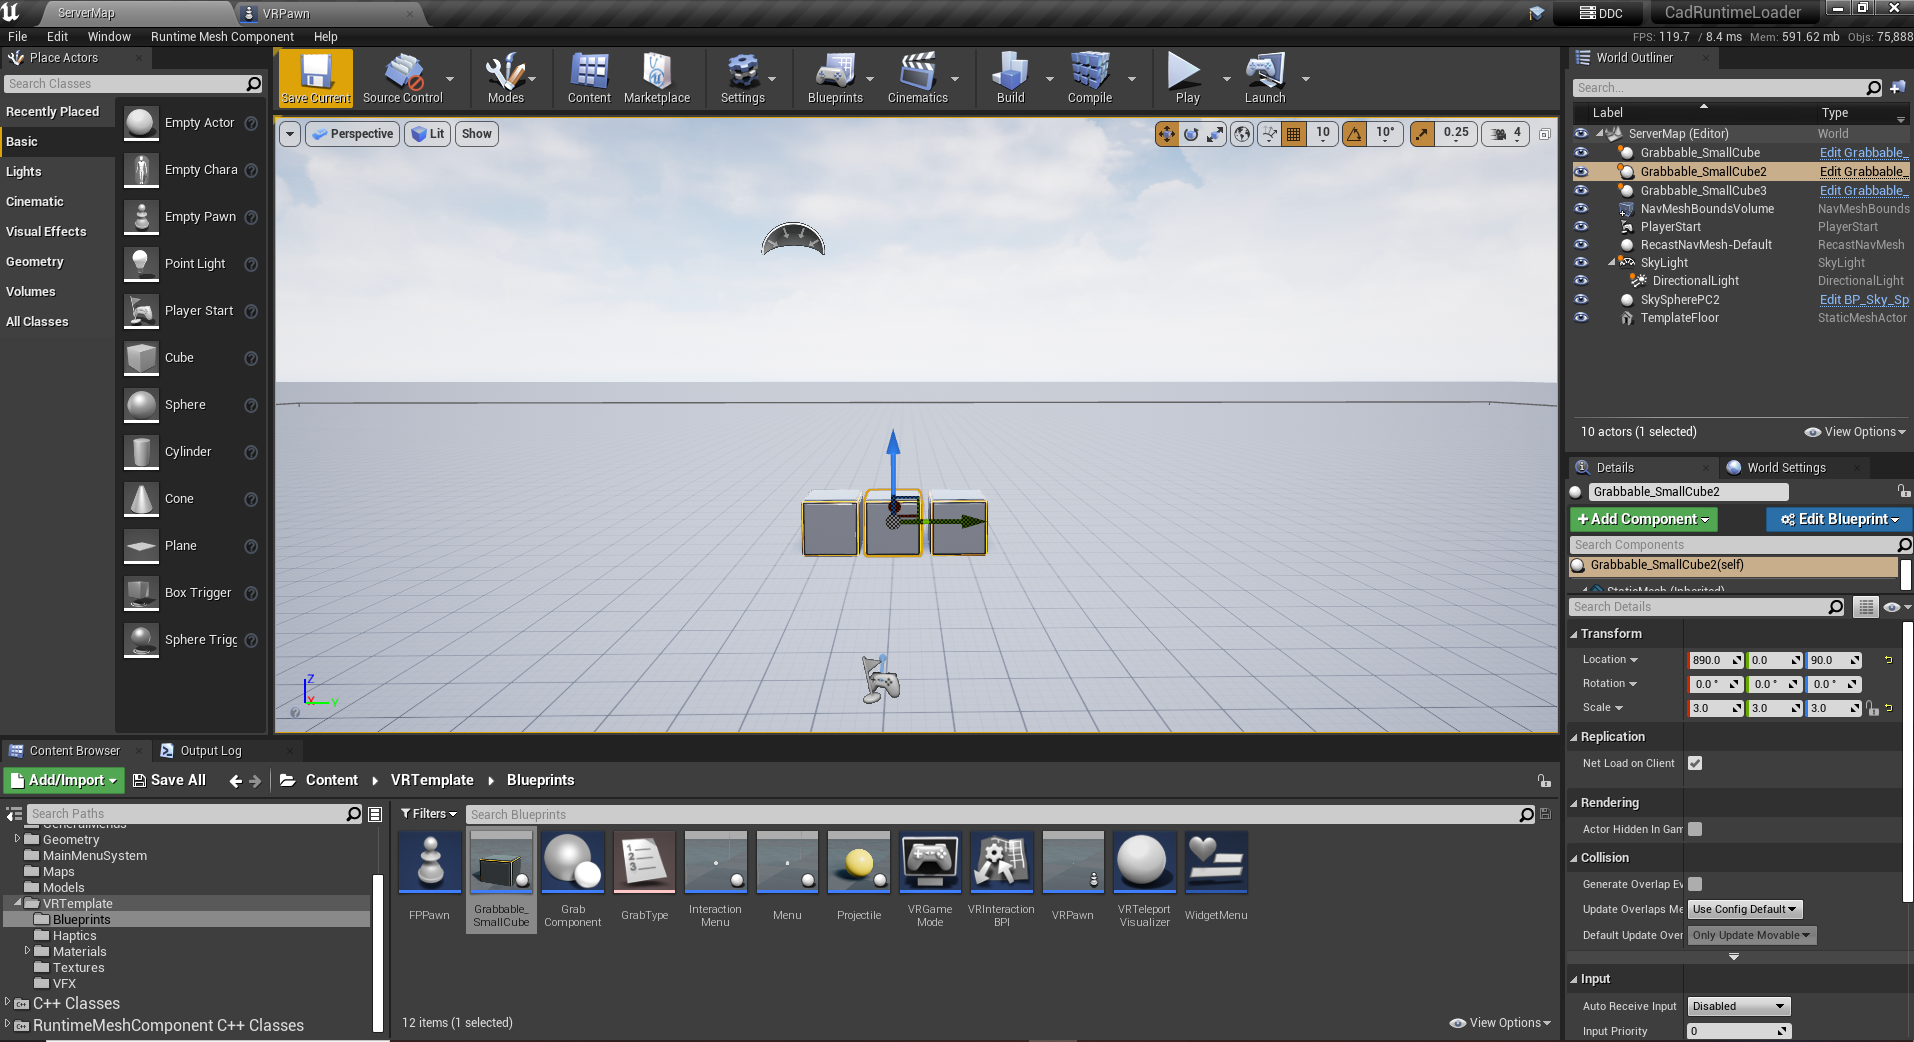
\includegraphics[width=0.9\textwidth]{fig/UnrealEngineLevelEditor.png}
	\caption[Unreal Engine Level Editor]{Example of what the Level Editor looks like for a project \protect}
	\label{fig:LevelEditor}
\end{figure}

\subsubsection{Actors and Components}

In Unreal Engine all of the objects that can be placed inside of a level are called Actors. This includes everything from meshes to particle systems to even the players starting location. This is partially due to Unreal Engines object-oriented nature so having all objects inherit from one base class, in this case Actor, is quite beneficial. Actors can be created and destroyed through code and support 3D transformations like translation, scaling and rotation.\\

In order to add functionality to an Actor, so called Components are used. Components can offer varying functionalities such as creating sounds, light or movement and once they are added to an Actor, the Actor can access these features and use them for its own purposes. It is important to note that a Component cannot exist on its own and an instance of a Component has to be attached to an instance of an Actor. It doesn't have to be directly attached though, a Component itself can also have several subcomponents. So the Components are what actually makes an Actor what it is supposed to be. One way to think about this is a house. All of the walls, floors, lights and other parts would be the Components, while the house in its entirety  is the Actor.\\

When an Actor is placed inside a level it gets a world transformation which describes the Actors location, scale and rotation in comparison to the world origin. A Component along with that also gets a relative transform, which are again the same values as the world transformation but this time relative to  the origin of its parent object. The world transform of a component can be calculating by adding the relative transformation to the parents world transformation. This is very important to keep in mind when components are moved around in a scene. 

\subsubsection{Pawns and Controllers}
Amongst all of the Actor subclasses, there are two which need to be especially highlighted. These are Pawns and Controllers and they form the basis of user-interaction in Unreal Engine.\\
The Pawn class is the base class for all Actors which can be controlled by a user or through AI. A Pawn determines what a user looks like visually and how they interact with their surroundings either through collision or other physical means. Generally for Pawns that will be controlled by users a further subclass called Character is used. A Character has the additions of a Character Movement, Capsule and Skeletal Mesh Component. The Character Movement Component enables various means of moving like walking, flying, swimming for a character in a scene. It assumes that collision class is vertically-oriented capsule, described in the Capsule Component, and uses this for movement collision. The Skeletal Mesh simply allows for the use of more complex animations which require some sort of skeleton. What this looks like inside the editor can be seen in Figure \ref{fig:UnrealCharacter}. This is the basic template Unreal provides for a third person character. Aside from the already mentioned components, it also has an Arrow Component, which shows what direction is forwards for the character, and a Camera Component that represents where the view of a user will be in a project.\\

\begin{figure}[htpb]
	\centering
	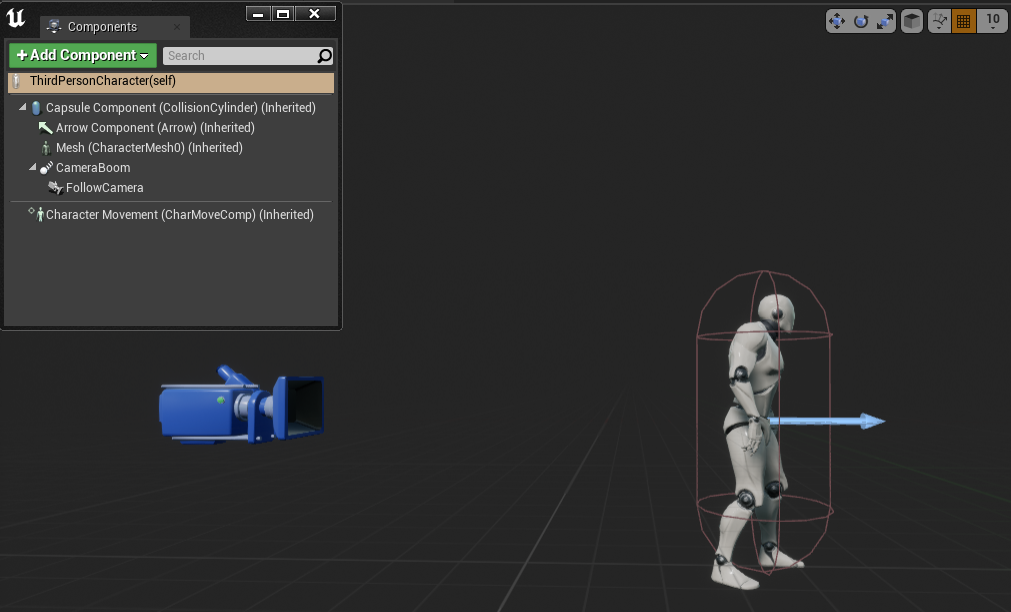
\includegraphics[width=0.9\textwidth]{fig/UnrealCharacter.png}
	\caption[Template for third person character]{Template for third person character\protect}
	\label{fig:UnrealCharacter}
\end{figure}

While some functionalities can already be implemented inside of a Pawn, this alone is not enough to get user inputs. For that an additional Actor called a Controller is necessary, specifically a Player Controller. A Player Controller is a non-physical Actor that functions as an interface between a human user and a Pawn. Generally speaking there is a one-to-one relationship between a Player Controller and a Pawn. There are cases where this doesn't have to be the case but for the purposes of this project that is not of interest. This relationship doesn't mean that a Controller can only ever posses one Pawn, just that it can only do one Pawn at a time. The process of gaining controller over a Pawn is called possessing and losing control is called unpossessing. This, alongside slight differences between classes, is why it is important to properly choose whether certain functionalities should be implemented in the Pawn or the Controller.

\section{C++ and Blueprints}

Now that the most important design elements have been explained, the next step is to explain how writing code in Unreal Engine works. When it comes to this regard, Unreal has a rather unique combination of programming tools with C++ and its own Blueprint Visual Scripting system. As already mentioned, Unreal is written in C++ so it makes sense that it would also be used for its programming. What is important to note is the fact that it is not pure C++ that is actually used. Rather, Unreal Engine has developed its own extensive C++ API, also known as simply Unreal C++, tailored for game development build upon normal C++. This API provides libraries for common game development features as well many built-in classes, functions and utilities. The idea behind this is to have a fully functioning framework that makes the developing process a lot simple and faster than it would've been using standard C++. An excellent example of this is the fact the Unreal C++ support multiplayer and network replication on a core engine level.\\

The other way to program in Unreal Engine is the Blueprint Visual Scripting system, more commonly referred as simply Blueprints. This system is a relatively new addition to Unreal as it was first released with the launch of Unreal Engine 4. It was meant to be a replacement for the previous Kismet scripting system which was quite complicated and very outdated. Blueprints themself, like many visual scripting languages, use an object-oriented approach for developing. It is a very powerful and flexible tool which is meant to allow designers to create impressive gameplay elements without needing to know how to program. As such it has access to almost all the same frameworks and APIs C++ has. This means that whole games and projects could be made only using blueprints. Likewise the same could also be done with only C++ but such approaches are generally not advised. There is a reason after all why Unreal specifically has both tools and they each have their purposes in development. C++ is advantageous when designing base systems for a project and for writing performance critical features. On the other hand, Blueprints shine when they are used to design the behaviour and incorporate it into the rest of the program. Another great benefit of Blueprints is that, due to their simplicity, allow for rapid prototyping and then these prototypes can easily be translated into C++ if the increased performance is necessary.\\
Due to this unique mix of tools, a typical workflow for creating features would look as follows. First a C++ programmer would create a new class, add the required features and properties and then make sure that they can properly be accessed in the Blueprints. An example of a header for such a class is shown in Figure \ref{fig:ClassExample}.
\begin{figure}[htpb]
	\centering
	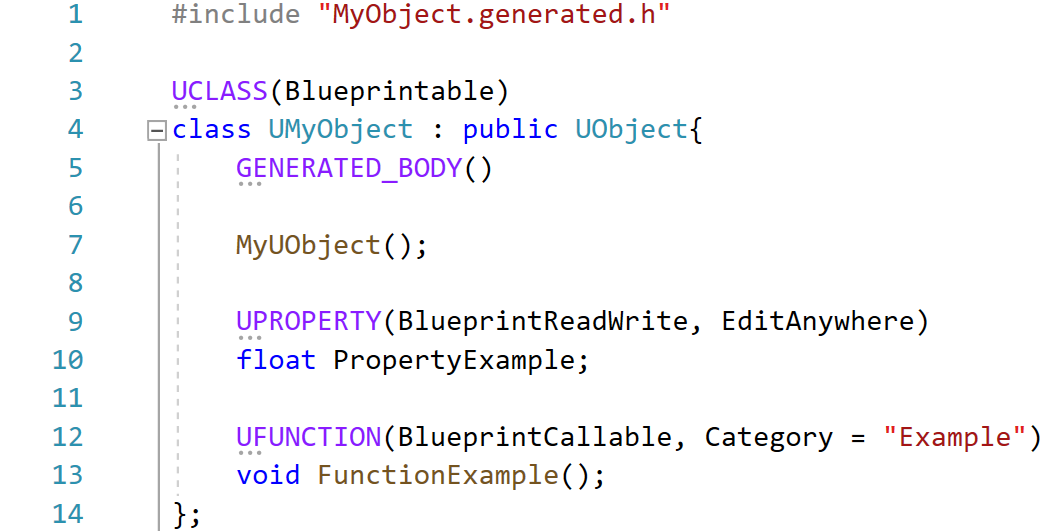
\includegraphics[width=0.8\textwidth,height=160pt]{fig/ClassExample3.png}
	\caption[Example Unreal C++ Class Header]{Example Unreal C++ Class Header\protect}
	\label{fig:ClassExample}
\end{figure}
As can be seen, the code does resemble normal C++ header code with a few special lines. Most important are the macros that can be found in the 3rd, 9th and 12th line of code. These special lines of code are used to describe the class, property or function in the line below them. This description is used by the Unreal Editor to determine if and how these objects should be presented in Blueprints. As an example the property is set to "BlueprintReadWrite" so that it can be read and modified in Blueprints. There are many specifiers that can be used depending on what the desired outcome is and it is important that these are used properly to mitigate possible problems.\\
 
Once that part of the development is done, the new class can be used in the engine. The class itself, seeing as it is C++ code, can't be directly worked with in the Blueprint editor. Instead a new Blueprint class needs to be made that inherits from the C++ class and then that new class can be opened in the editor.\\
As already mentioned, Blueprints are a visual scripting system, which means that the code isn't represented through text but rather with nodes which are connected among each other. An example as to how this looks like in the Blueprint editor is shown in Figure \ref{fig:BlueprintExample}.

\begin{figure}[htpb]
	\centering
	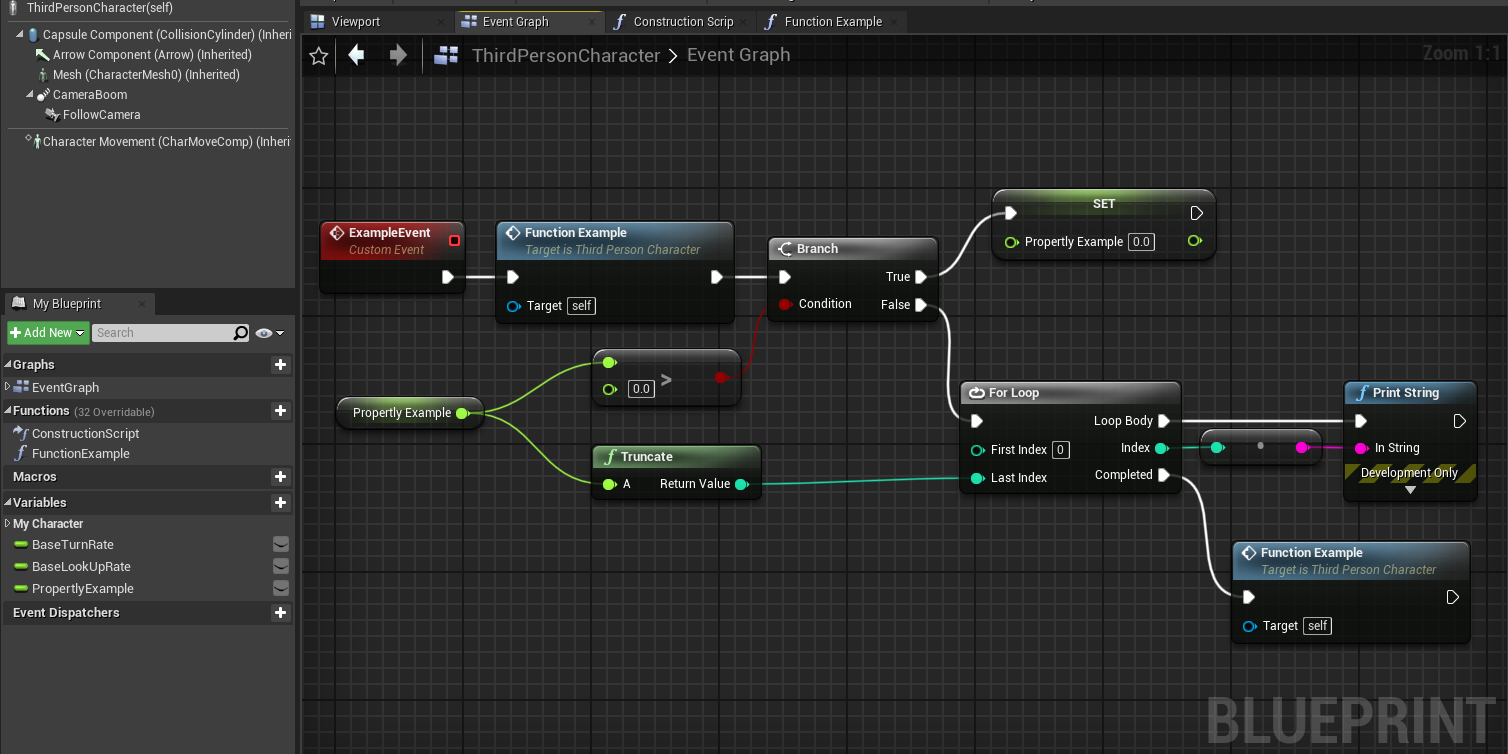
\includegraphics[width=0.9\textwidth]{fig/BlueprintExample.png}
	\caption[Example Blueprint Code]{Example of Blueprint Code in the Blueprint Editor\protect}
	\label{fig:BlueprintExample}
\end{figure}

In the top left side of the screen the components of the current actor can be seen again. Underneath that is an overview of all the functions, graphs and variables contained in the blueprint. In the centre of the editor is the event graph of the class, this is where all the various events that can happen to it are handled. In the example shown it needs to be noted that the view is heavily zoomed into a single event in order to better see the individual nodes. Typically there will be many events all across the graph and also sub-graphs to keep the code readable.\\
The execution flow of the code is represented by the white line connecting the nodes. The nodes themselves have varying functions and are accordingly colour coded for better understanding. Red nodes represent the starting point of an event. This can be triggered by many actions including collision, player inputs or other events. Blue nodes are either functions or event calls and green nodes are usually used for getting values. Lastly grey nodes represent macros or flow control nodes. This is where the typical programming tools such as if conditions, for and while loops can be found.
Depending on if they are needed, input and output pins can respectively be found on the left and right side of a node. These are connected using lines that automatically match the colour of the value, which are also colour coded, and can only be connected to other pins of the correct type.\\
All in all, these properties and features make using Blueprints quite simple and almost play-like, which makes them accessible to a wider audience, while staying quite powerful.

\section{Networking}

Everything that was discussed so far mostly relates to what happens in a single instance of our program. Nonetheless, as already mentioned, networking is a big part of Unreal Engine and is required to understand the steps that are needed in order to create a multi-user project.\\

When the program runs in a standalone mode, all of the objects that make it up exist on the local machine which is running the program and only that machine. For a network multi-user program, Unreal Engine uses a so-called client server model. One computer acts as a server and hosts a session that can be joined by other user as clients. The server is what connects all of the different users and enables their communication with each other. The instance running on the server is the true, authoritative world instance. In order words this is where the multiplayer is actually happening. The clients only have copies of this world. The server dictates the clients what Actors exist, how they should behave and values their variables should have. The clients then use this information to approximate what is happening on the server in their own copy of the world. The clients only really control the Pawn and Player controller that they are assigned to. One thing to note is that while a copy of a Pawn exists in every instance of the program, the Player Controller only exists for the owning player and server. This means that a local Player Controller is completely unaware of the existence of other Player Controllers.\\

In total there are three network modes in which an Unreal project can run in: standalone, client and server. For the server mode there is a further classification into listen and dedicated servers. A listen server represents a user hosting a session through their local machine. This means that they function both as a server and a client simultaneously. The benefit of this is its relative simplicity, especially with Unreals already existing tools and support for many popular online subsystems such as Google, Amazon and Steam. A big downside of this approach is the extra load that is put on the server machine, as it also has to handle user-relevant features like graphics. Also the user that hosts the server can get a slight advantage from the non-existent latency, although this is only relevant in specific use-case.\\
A dedicated server on the other hand runs "headlessly", which means it does not have to render any visuals and isn't controlled by anyone locally. This means that most of the resources available to the machine can be used for hosting and moderating the program. Unfortunately this requires a separate computer with its own network connection, not to mention a lot of complex work to be properly configured.\\

\begin{figure}[htpb]
	\centering
	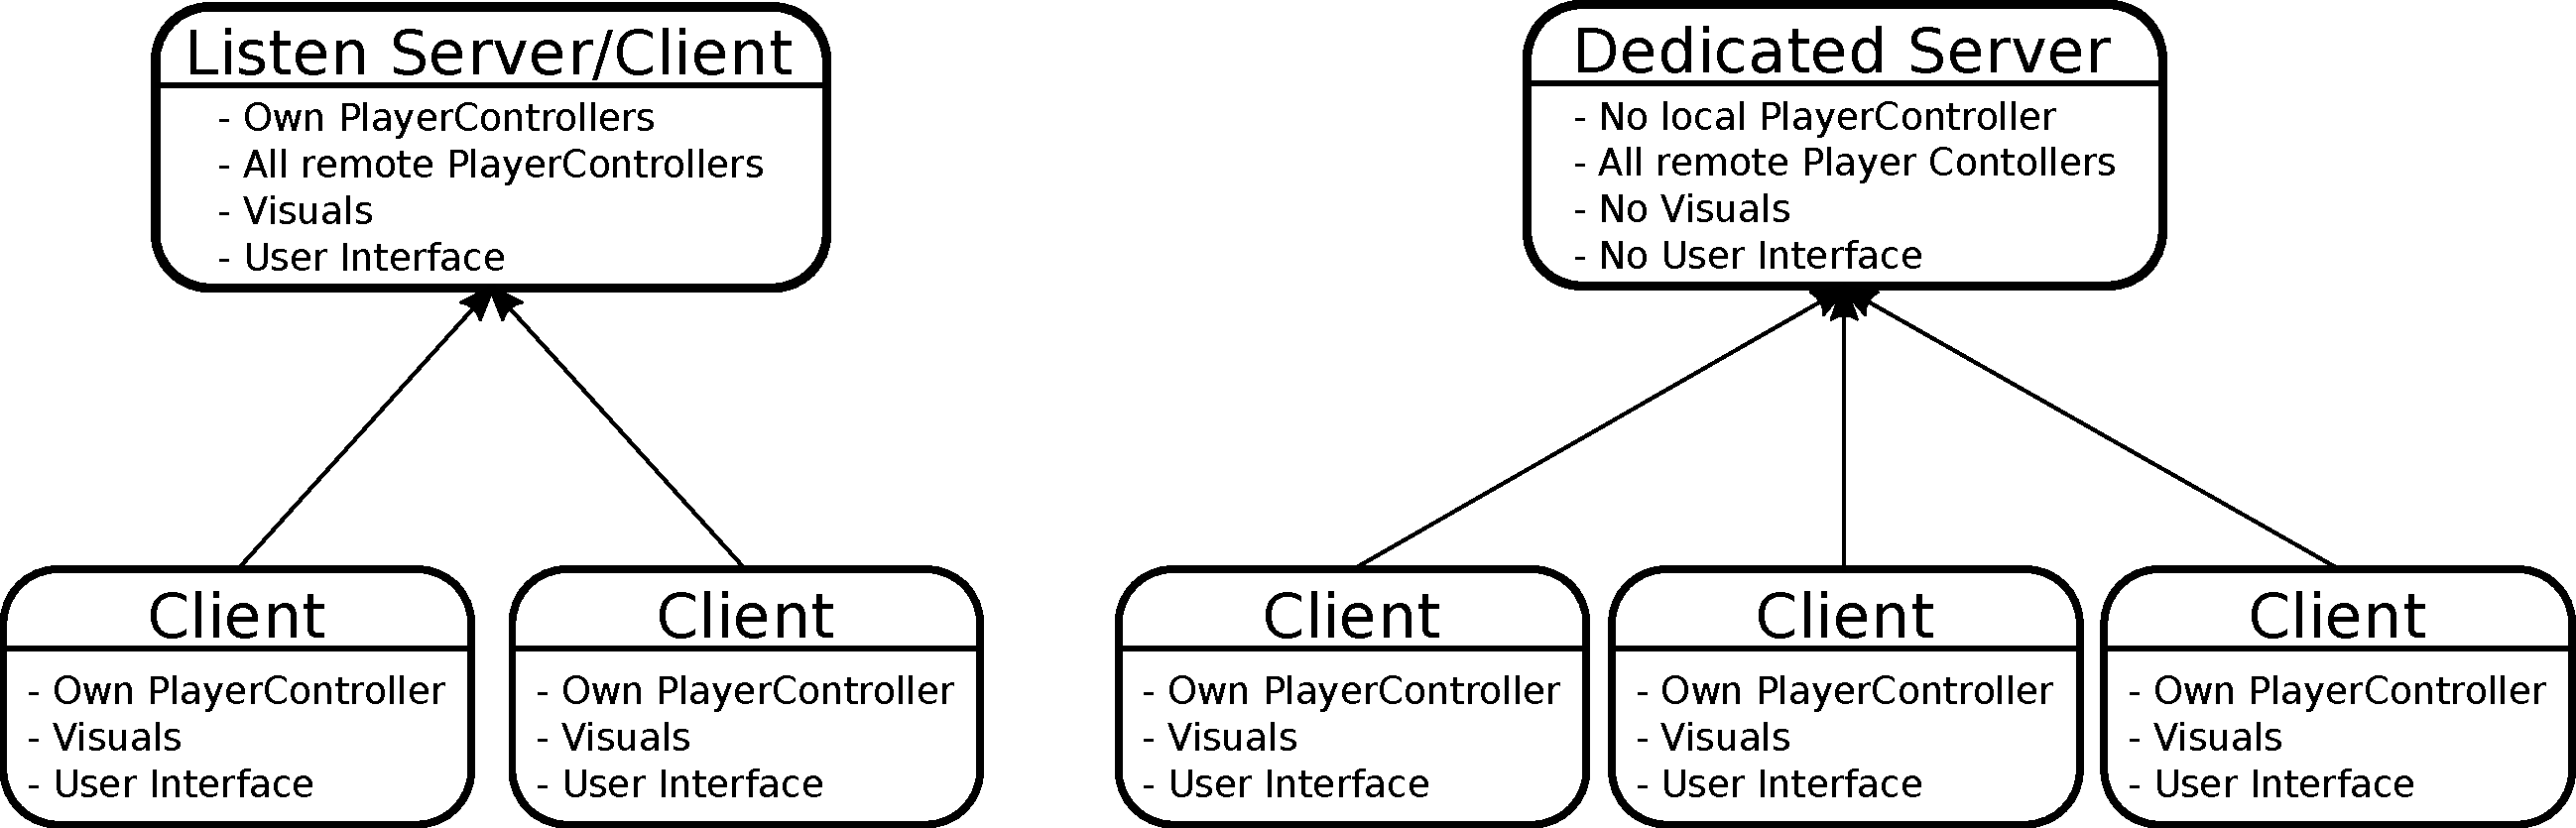
\includegraphics[width=1\textwidth]{fig/ListenvsDedicated.pdf}
	\caption[Difference between Listen and Dedicated Server]{Example to demonstrate differences between a Listen and Dedicated server\protect}
	\label{fig:ListenvDedicated}
\end{figure}

The actual information sharing and interaction between users through a server is done through replication and remote procedure calls. In order to use replication for a variable, its boolean specifier "Replicated" needs to be set to true. Now when the variable's value is changed on an authoritative Actor, usually on the server, the change is automatically sent to the connected remote copies of the Actor. Likewise if a variable is changed locally in a clients instance, this will not be replicated to the server or other clients. This doesn't mean that every variable needs to be replicated, as that could cause problems in network traffic. Rather it is important to use replication carefully and replicate only variables that require it.\\
Remote procedure calls(RPCs) are functions which are called from a machine but executed remotely on another machine. They are also known as replicated functions. In order for a function to become an RPC, the keywords server, client or multicast need to be added to its definition. The server and client keywords simply mean that the function should be executed on specifically on the server or client. Multicast means that a function will be called on every instance of an object. Another peculiarity of RPCs is that they have no return value. In order to achieve that another RPC is needed which returns the output from the remote to the local machine.\\
All of this is only a small section of all the features that Unreal Engine is capable of but for the purposes of this project this should suffice as an introduction to the engine and make understanding the rest of the work easier.




% replications, rpcs,